% Options for packages loaded elsewhere
\PassOptionsToPackage{unicode}{hyperref}
\PassOptionsToPackage{hyphens}{url}
\PassOptionsToPackage{dvipsnames,svgnames,x11names}{xcolor}
%
\documentclass[
]{agujournal2019}

\usepackage{amsmath,amssymb}
\usepackage{iftex}
\ifPDFTeX
  \usepackage[T1]{fontenc}
  \usepackage[utf8]{inputenc}
  \usepackage{textcomp} % provide euro and other symbols
\else % if luatex or xetex
  \usepackage{unicode-math}
  \defaultfontfeatures{Scale=MatchLowercase}
  \defaultfontfeatures[\rmfamily]{Ligatures=TeX,Scale=1}
\fi
\usepackage{lmodern}
\ifPDFTeX\else  
    % xetex/luatex font selection
\fi
% Use upquote if available, for straight quotes in verbatim environments
\IfFileExists{upquote.sty}{\usepackage{upquote}}{}
\IfFileExists{microtype.sty}{% use microtype if available
  \usepackage[]{microtype}
  \UseMicrotypeSet[protrusion]{basicmath} % disable protrusion for tt fonts
}{}
\makeatletter
\@ifundefined{KOMAClassName}{% if non-KOMA class
  \IfFileExists{parskip.sty}{%
    \usepackage{parskip}
  }{% else
    \setlength{\parindent}{0pt}
    \setlength{\parskip}{6pt plus 2pt minus 1pt}}
}{% if KOMA class
  \KOMAoptions{parskip=half}}
\makeatother
\usepackage{xcolor}
\setlength{\emergencystretch}{3em} % prevent overfull lines
\setcounter{secnumdepth}{5}
% Make \paragraph and \subparagraph free-standing
\ifx\paragraph\undefined\else
  \let\oldparagraph\paragraph
  \renewcommand{\paragraph}[1]{\oldparagraph{#1}\mbox{}}
\fi
\ifx\subparagraph\undefined\else
  \let\oldsubparagraph\subparagraph
  \renewcommand{\subparagraph}[1]{\oldsubparagraph{#1}\mbox{}}
\fi


\providecommand{\tightlist}{%
  \setlength{\itemsep}{0pt}\setlength{\parskip}{0pt}}\usepackage{longtable,booktabs,array}
\usepackage{calc} % for calculating minipage widths
% Correct order of tables after \paragraph or \subparagraph
\usepackage{etoolbox}
\makeatletter
\patchcmd\longtable{\par}{\if@noskipsec\mbox{}\fi\par}{}{}
\makeatother
% Allow footnotes in longtable head/foot
\IfFileExists{footnotehyper.sty}{\usepackage{footnotehyper}}{\usepackage{footnote}}
\makesavenoteenv{longtable}
\usepackage{graphicx}
\makeatletter
\def\maxwidth{\ifdim\Gin@nat@width>\linewidth\linewidth\else\Gin@nat@width\fi}
\def\maxheight{\ifdim\Gin@nat@height>\textheight\textheight\else\Gin@nat@height\fi}
\makeatother
% Scale images if necessary, so that they will not overflow the page
% margins by default, and it is still possible to overwrite the defaults
% using explicit options in \includegraphics[width, height, ...]{}
\setkeys{Gin}{width=\maxwidth,height=\maxheight,keepaspectratio}
% Set default figure placement to htbp
\makeatletter
\def\fps@figure{htbp}
\makeatother
% definitions for citeproc citations
\NewDocumentCommand\citeproctext{}{}
\NewDocumentCommand\citeproc{mm}{%
  \begingroup\def\citeproctext{#2}\cite{#1}\endgroup}
\makeatletter
 % allow citations to break across lines
 \let\@cite@ofmt\@firstofone
 % avoid brackets around text for \cite:
 \def\@biblabel#1{}
 \def\@cite#1#2{{#1\if@tempswa , #2\fi}}
\makeatother
\newlength{\cslhangindent}
\setlength{\cslhangindent}{1.5em}
\newlength{\csllabelwidth}
\setlength{\csllabelwidth}{3em}
\newenvironment{CSLReferences}[2] % #1 hanging-indent, #2 entry-spacing
 {\begin{list}{}{%
  \setlength{\itemindent}{0pt}
  \setlength{\leftmargin}{0pt}
  \setlength{\parsep}{0pt}
  % turn on hanging indent if param 1 is 1
  \ifodd #1
   \setlength{\leftmargin}{\cslhangindent}
   \setlength{\itemindent}{-1\cslhangindent}
  \fi
  % set entry spacing
  \setlength{\itemsep}{#2\baselineskip}}}
 {\end{list}}
\usepackage{calc}
\newcommand{\CSLBlock}[1]{\hfill\break\parbox[t]{\linewidth}{\strut\ignorespaces#1\strut}}
\newcommand{\CSLLeftMargin}[1]{\parbox[t]{\csllabelwidth}{\strut#1\strut}}
\newcommand{\CSLRightInline}[1]{\parbox[t]{\linewidth - \csllabelwidth}{\strut#1\strut}}
\newcommand{\CSLIndent}[1]{\hspace{\cslhangindent}#1}

\usepackage{url} %this package should fix any errors with URLs in refs.
\usepackage{lineno}
\usepackage[inline]{trackchanges} %for better track changes. finalnew option will compile document with changes incorporated.
\usepackage{soul}
\linenumbers
\makeatletter
\@ifpackageloaded{caption}{}{\usepackage{caption}}
\AtBeginDocument{%
\ifdefined\contentsname
  \renewcommand*\contentsname{Table of contents}
\else
  \newcommand\contentsname{Table of contents}
\fi
\ifdefined\listfigurename
  \renewcommand*\listfigurename{List of Figures}
\else
  \newcommand\listfigurename{List of Figures}
\fi
\ifdefined\listtablename
  \renewcommand*\listtablename{List of Tables}
\else
  \newcommand\listtablename{List of Tables}
\fi
\ifdefined\figurename
  \renewcommand*\figurename{Figure}
\else
  \newcommand\figurename{Figure}
\fi
\ifdefined\tablename
  \renewcommand*\tablename{Table}
\else
  \newcommand\tablename{Table}
\fi
}
\@ifpackageloaded{float}{}{\usepackage{float}}
\floatstyle{ruled}
\@ifundefined{c@chapter}{\newfloat{codelisting}{h}{lop}}{\newfloat{codelisting}{h}{lop}[chapter]}
\floatname{codelisting}{Listing}
\newcommand*\listoflistings{\listof{codelisting}{List of Listings}}
\makeatother
\makeatletter
\makeatother
\makeatletter
\@ifpackageloaded{caption}{}{\usepackage{caption}}
\@ifpackageloaded{subcaption}{}{\usepackage{subcaption}}
\makeatother
\ifLuaTeX
  \usepackage{selnolig}  % disable illegal ligatures
\fi
\usepackage{bookmark}

\IfFileExists{xurl.sty}{\usepackage{xurl}}{} % add URL line breaks if available
\urlstyle{same} % disable monospaced font for URLs
\hypersetup{
  pdftitle={From Precipitation to Prediction: Integrating ConvLSTM Models for Comprehensive River Runoff Forecasting},
  pdfauthor={Florian Börgel; Sven Karsten; Karoline Rummel},
  colorlinks=true,
  linkcolor={blue},
  filecolor={Maroon},
  citecolor={Blue},
  urlcolor={Blue},
  pdfcreator={LaTeX via pandoc}}

\journalname{Climate Dynamics}

\draftfalse

\begin{document}
\title{From Precipitation to Prediction: Integrating ConvLSTM Models for
Comprehensive River Runoff Forecasting}

\authors{Florian Börgel\affil{1}, Sven Karsten\affil{1}, Karoline
Rummel\affil{1}}
\affiliation{1}{Leibniz-Institute for Baltic Sea Research Warnemünde, }
\correspondingauthor{Florian Börgel}{florian.boergel@io-warnemuende.de}


\begin{abstract}
a
\end{abstract}

\section*{Plain Language Summary}
b



\section{Introduction}\label{introduction}

River runoff is an important component of the global water cycle as it
comprises about one third of the precipitation over land areas (Hagemann
et al., 2020). In the context of climate change studies, river runoff is
usually generated in two ways. First, river runoff as input for ocean
models can be created using hyrdological models such as the Hydrological
Discharge (HD) model (Hagemann et al., 2020). HD models calculates the
water balance using hydrological processes (e.g.~snow, glaciers, soil
moisture, groundwater contribution). It represents a complex forecasting
tool that uses underlying physical processes. A different approach would
use data-based models that intergrate statistical correction, using the
land surface schemes of global or regional climate models.

The releatively recent rise of machine learning (ML) models has been
mostly explored for river runoff forecasting, as accurate runoff
forecasting, especially over extended periods, is pivotal for effective
water resources management (Fang et al., 2019; Tan et al., 2018; Yang et
al., 2018). Common approaches employ artificial neural networks, support
vector machines, adaptive neuro-fuzzy inference systems, and notably,
Long Short-Term Memory (LSTM) neural networks that have gained traction
for long-term hydrological forecasting due to their excellent
performance (Humphrey et al 2016, Huang et al 2014, Ashrafi et al 2017,
Yuan et al 2018, Xu et al 2021).

LSTM networks, an evolution of the classical Recurrent Neural Networks
(RNNs), have shown stability and efficacy in sequence-to-sequence
predictions, such as using climatic indices for rainfall estimation or
long-term hydrological forecasting. However, a limitation of LSTMs is
their inability to effectively capture two-dimensional structures, an
area where Convolutional Neural Networks (CNNs) excel. Reconizing this
limitation (SHI et al., 2015) proposed a convolutional LSTM (ConvLSTM)
architectures, which combines the strengths of both LSTM and CNN. The
ConvLSTM network has been proven useful for precipitation nowcasting
(SHI et al., 2015) or for river runoff forecasting {[}Ha et al. (2021);
@niu2020{]}.

In the following we will show that in absence of a fully functioning
hydrogolocial model, that also uses a rather complex parametrization,
ConvLSTM also represent a robust way to predict multiple rivers at once
for any given period using only atmospheric forcing. In this work we use
the Baltic Sea catchment to illustrate our approach, while in principal
the methodology we propose is universally applicable across various
geographic regions. The Baltic Sea serves as a challenging example due
to its unique hydrological characteristics, being nearly decoupled from
the open ocean (see Figure). As a consequence, the salinity of the
Baltic Sea is driven to a large part by freshwater supply from rivers.
More generally, the freshwater input into the Baltic Sea comes either as
river runoff or a positive net precipitation (precipitation minus
evaporation) over the sea surface. The net precipitation accounts for 11
\% and the river input for 89 \% of the total freshwater input (Meier
and Doescher, 2002). Modeling the Baltic Sea is therefore to a large
part the result of the quality of the river input, that is used for the
simulation. This makes the accurate modeling of river runoff especially
critical for simulations pertaining to the Baltic Sea.

In this work we will, we present a ConvLSTM architecture that is able to
predict daily river runoff for 97 rivers across the Baltic Sea
catchment.

\section{Methods}\label{methods}

\subsection{Runoff data used for
training}\label{runoff-data-used-for-training}

The runoff data covering the period 1979 to 2011 is based on an E-HYPE
hindcast simulation that was forced by a regional downscaling of
ERA-Interim (Dee et al., 2011) with RCA3 ({``The rossby centre regional
climate model RCA3,''} n.d.) and implemented into NEMO-Nordic (Hordoir
et al., 2019) as a mass flux. For the periods before (1961 to 1978) and
after (2012 to 2018) additional spatial temporal corrections have been
applied to the runoff data, and have therefore been ignored. For more
information see Gröger et al. (2022) and references therein.

\subsection{Atmospheric Forcing}\label{atmospheric-forcing}

The UERRA-HARMONIE regional reanalysis dataset was developed as part of
the FP7 UERRA project (Uncertainties in Ensembles of Regional
Re-Analyses, \href{http://www.uerra.eu/}{http://www.uerra.eu/)},). The
UERRA-HARMONIE system represents a comprehensive, high-resolution
reanalysis covering a wide range of essential climate variables. This
dataset encompasses data on air temperature, pressure, humidity, wind
speed and direction, cloud cover, precipitation, albedo, surface heat
fluxes, and radiation fluxes from January 1961 to July 2019. With a
horizontal resolution of 11 km and analyses conducted at 00 UTC, 06 UTC,
12 UTC, and 18 UTC, it also provides hourly resolution forecast model
data. UERRA-HARMONIE is accessible through the Copernicus Climate Data
Store (CDS, \url{https://cds.climate.copernicus.eu/\#!/home),} initially
produced during the UERRA project and later transitioned to the
Copernicus Climate Change Service (C3S,
\url{https://climate.copernicus.eu/copernicus-regionalreanalysis-europe).}

\subsection{Ocean Model}\label{ocean-model}

To simulate the Baltic Sea, we use a coupled 3-dimensional ocean model
Baltic Sea, called the Modular Ocean Model (MOM). This model uses a
finite-difference method to solve the full set of primitive equations to
calculate the motion of water and the transport of heat and salt. The
K-profile parameterization (KPP) was used as turbulence closure scheme.
The model's western boundary opens into the Skagerrak and connects the
Baltic Sea to the North Sea. The maximum depth was set at 264 meters. A
more detailed description of the setup can be found in (Gröger et al.,
2022).

\subsection{LSTM network}\label{lstm-network}

Before turning to the convolutional LSTM, the simpler architecture of
the plain LSTM is examined and should serve as a role model for the
later consideration of the full ConvLSTM.

The Long Short-Term Memory (LSTM), a specialized form of Recurrent
Neural Networks (RNNs), is specifically tailored for modeling temporal
sequences
\(\vec{X}^t[1], \ldots \vec{X}^t[\tau],\ldots \vec{X}^t[N_\tau]\) of
\(N_\tau\) input quantities
\(\vec{X}^t[\tau] = (X^t_k[\tau]) \in \mathbb{R}^{N_k}\). The sequence
is taken from a dataset given in form of a time series \(\{\vec{X}^t\}\)
and the endpoint should coincide with the specific element in the time
series connected to time \(t\),
i.e.~\(\vec{X}^t[N_\tau] \equiv \vec{X}^t\). The \(N_k\) is the number
of used input ``channels'' and can, for example, represent different
measurable quantities. Its unique design allows it to adeptly handle
long-range dependencies, setting it apart from traditional RNNs in terms
of accuracy (see Figure~\ref{fig-lstm}).

\begin{figure}

\centering{

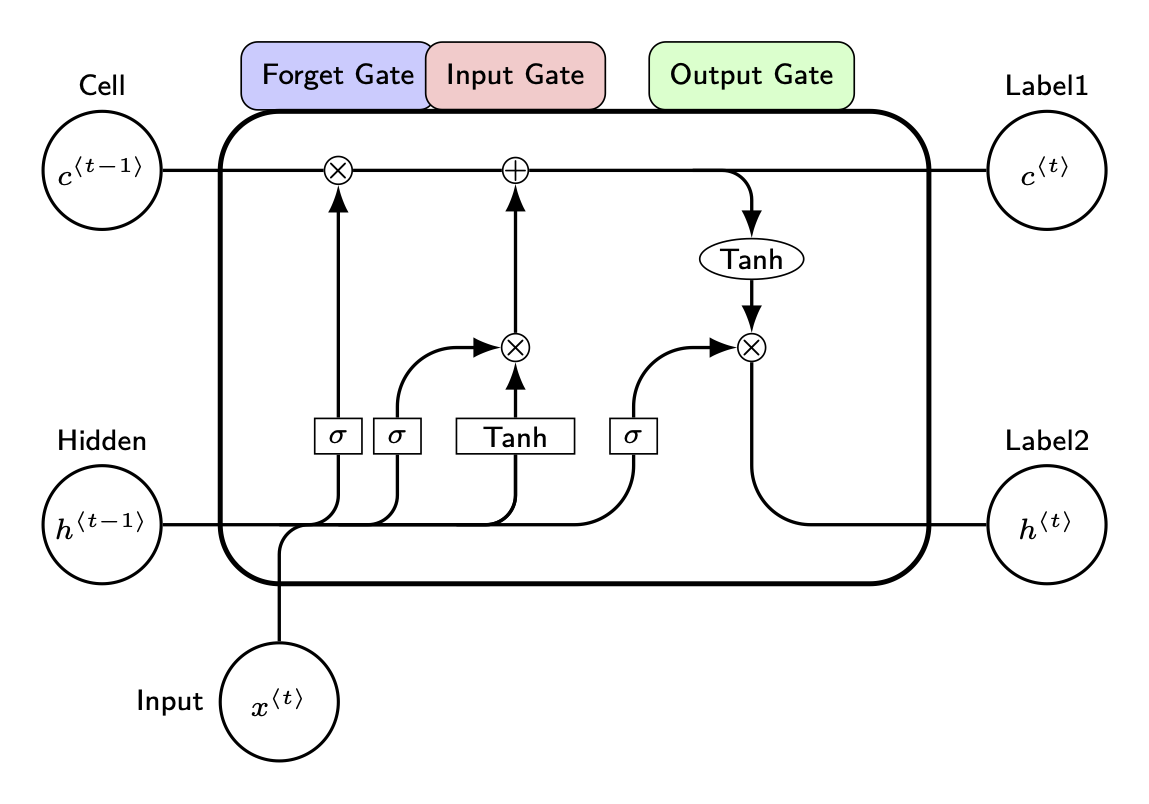
\includegraphics{draw_lstm.png}

}

\caption{\label{fig-lstm}Inner structure of a Long Short-Term Memory
Cell}

\end{figure}%

This performance in modeling long-range dependencies has been validated
in various studies. The key component of LSTM's innovation is its memory
cell, \(\vec{C}^t[\tau] = (C^t_h[\tau]) \in \mathbb{R}^{N_h}\), which
stores state information, also referred to as long-term memory. The
index \(\tau \in [1, N_\tau]\) corresponds to the \(\tau\)-th element in
the input sequence. The cell state is a vector consists of elements,
each associated with one of the \(N_h\) hidden layers, labeled by \(h\).
This vector is determined through several self-parameterized gates, all
in the same vector space as \(\vec{C}^t[\tau]\). The forget gate
\(\vec{F}^t[\tau]\) defines the percentage of the previous long-term
memory status \(\vec{C}^t[\tau-1]\) that should be retained
stored\hspace{0pt}. The input gate \(\vec{I}^t[\tau]\) decides how much
of the input is added to the the long-term memory, forming the updated
cell state. The so-called output gate \(\vec{O}^t[\tau]\) then
determines how much of the latest cell output, \(\vec{C}^t[\tau]\), is
propagated to the final state, \(\vec{H}^t[\tau]\) representing the
updated short-term memory of the hidden state.

For a fixed point \(\tau\) in the sequence, the action of a LSTM cell,
i.e.~the connection between the input \(\vec{X}^t[\tau]\), the various
gates and the state vectors, is given as follows. First, the elements of
the input sequence together with the hidden state are mapped onto
auxiliary gate vectors, collectively denoted by
\(\vec{g}^t[\tau] = (g^t_h[\tau]) \in \mathbb{R}^{N_h}\), via \[
\begin{aligned}
g_h^t[\tau] =  \mathcal{M}^{g}_{hk} \, X^t_k[\tau] +  \mathcal{N}^{g}_{hh'} \, H^t_{h'}[\tau-1] + \mathcal{B}^g_{h} \ ,
\end{aligned}
\]

where \(g=i,f,o,c\) stands for the input, forget, output and cell-state
gate, respectively and Eistein's summation convention is employed,
i.e.~indices that appear twice are summed over. The calligraphic symbols
\(\mathcal{M}^{g}_{hk}, \mathcal{N}^{g}_{hh'}\) and
\(\mathcal{B}^g_{h}\) are the free parameters of the network that are
optimized for the given problem during the training, which is at the
heart of the any machine learning approach. The matrix
\(\pmb{\mathcal{M}}^{g} = (\mathcal{M}^{g}_{hk}) \in \mathbb{R}^{N_h \times N_k}\)
can be interpreted as a Markovian-like contribution of the current input
\(\vec{X}^t[\tau]\) to the gates, whereas the
\(\pmb{\mathcal{N}}^{g} = (\mathcal{N}^{g}_{hh'}) \in \mathbb{R}^{N_h \times N_h}\)
scales a non-Markovian part determined by the hidden state of the last
sequence point \(\tau-1\). The vector
\(\vec{\mathcal{B}}^g = (\mathcal{B}^g_{h}) \in \mathbb{R}^{N_h}\) is a
learnable bias. It should be stressed that these parameters do neither
depend on \(t\) nor on \(\tau\) and are thus optimized once for the
complete dataset \(\{\vec{X}^t\}\).

Note that this mapping is sometimes extended by a contribution to the
\(g_h^t[\tau]\) from the past cell state \(\vec{C}^t[\tau-1]\)
(\textbf{XXX?}). Nevertheless, this mechanism called ``peeping'' is not
further considered in this work.

For the sake of brevity, we write the mapping more compactly in
matrix-vector form as
\begin{equation}\phantomsection\label{eq-LSTM-gates}{
\begin{aligned}
\vec{g}^t[\tau] = \pmb{\mathcal{M}}^{g}\vec{X}^t[\tau] + \pmb{\mathcal{N}}^{g}  \vec{H}^t[ \tau-1]+ \vec{\mathcal{B}}^g \,
\end{aligned}
}\end{equation}

Second, the actual gate vectors are computed by the core equations of
the LSTM as proposed by (\textbf{XXX?}):

\begin{equation}\phantomsection\label{eq-LSTM}{
\begin{aligned}
\vec{I}^t[\tau] &= \sigma(\vec{i}^t[\tau]) \\
\vec{F}^t[\tau] &= \sigma(\vec{f}^t[\tau]) \\
\vec{O}^t[\tau] &= \sigma(\vec{o}^t[\tau]) \\
\vec{C}^t[\tau] &= \vec{F}^t[\tau] \circ \vec{C}^t[\tau-1]  + \vec{I}^t[\tau] \circ \tanh(\vec{c}^t[\tau]) \\
\vec{H}^t[\tau]  &= \vec{O}^t[\tau] \circ \tanh(\vec{C}^t[\tau]) \ ,
\end{aligned}
}\end{equation}

where \(\sigma\) denotes the logisitc sigmoid function, \(\tanh\) is the
hyperbolic tangent and the \(\circ\) stands for the Hadamard product
(all applied in an element-wise fashion to the vectors). In the last two
equations the role of the input, forget and output gates as described
above become apparent.

The third step in a single layer LSTM (as employed for the work
presented here) is then to provide the output of the current LSTM cell,
i.e.~\(\vec{H}^t[\tau]\) and \(\vec{C}^t[\tau]\), to the subsequent LSTM
cell that processes the next element \(\vec{X}^t[\tau+1]\) of the input
sequence.

The full action of the LSTM network up to the end of the sequence can
therefore be written as a nested function call

\[
\left(\vec{H}^t[N_\tau], \vec{C}^t[N_\tau] \right) = L \left( \vec{X}^t[N_\tau], L \left( \vec{X}^t[N_\tau-1], \ldots L \left( \vec{X}^t[1], (\vec{H}^t[0], \vec{C}^t[0] \right) \ldots \right) \right) \ ,
\]

where \(L\) represents Eqs. (Equation~\ref{eq-LSTM-gates},
Equation~\ref{eq-LSTM}) and the initial conditions are usually chosen as
\(\vec{H}^t[0]=\vec{C}^t[0]=0\).

The final output \(\vec{H}^t[N_\tau]\) and \(\vec{C}^t[N_\tau]\) encode
information on the full input sequence ending at time \(t\). This
information has to be decoded to obtain usueful information via an
appropriate subsequent layer, as it is described in the Sec.
(\textbf{XXX?}).

A significant advantage of this architecture is the memory cell's
ability to retain gradients. This mechanism addresses the vanishing
gradient problem, where, as input sequences elongate, the influence of
initial stages becomes harder to capture, causing gradients of early
input points to approach zero. The LSTM's activation function,
inherently recurrent, mirrors the identity function with a consistent
derivative of 1.0, ensuring the gradient remains stable throughout
backpropagation.

\subsection{ConvLSTM network}\label{convlstm-network}

Although the plain LSTM has high performance in handling temporal
sequences of point-like quantities it is not designed to recognize
spatial features in seuqences of two-dimensional maps. To adress this
limitation we use a convLSTM architecture.

In this kind of network the elements of the input sequence are given as
(kind of) vector fields
\(\vec{X}^t[\tau] = (X^t_k[x,y,\tau]) \in \mathbb{R}^{N_k \times (N_x \times N_y)}\),
where \(x\in[1, N_x]\) and \(y \in [1, N_y]\) run over the horizontal
and vertical dimensions of the map, respectively. In order to enable the
``learning'' of spatial patterns, the free parameters of the network are
replaced by two-dimenmsional convolutional kernels
\(\pmb{\mathcal{M}}^{g} = (\mathcal{M}^{g}_{hk}[\xi, \eta]) \in \mathbb{R}^{(N_h \times N_k)\times (N_\xi \times N_\eta)}\)
and
\(\pmb{\mathcal{N}}^{g} = (\mathcal{N}^{g}_{hh'}[\xi, \eta]) \in \mathbb{R}^{(N_h \times N_h)\times (N_\xi \times N_\eta)}\).
The width and the height of the kernels are given by \(N_\xi\) and
\(N_\eta\), respectively and
\(\xi\in [-(N_\xi-1)/2,(N_\xi-1)/2], \eta\in [-(N_\eta-1)/2,(N_\eta-1)/2]\),
where we assume odd numbers for the kernel sizes.

The mapping from the input quantities to the gates is then given by a
convolution with these kernels \[
\begin{aligned}
g^t_h[x,y,\tau] & =  \mathcal{M}^{g}_{hk} [\xi,\eta]\, X^t_k[x-\xi, y-\eta, \tau]  +  \mathcal{N}^{g}_{hh'}[\xi,\eta] \, H^t_{h'}[x-\xi, y-\eta, \tau-1] + \mathcal{B}^g_{h}[x,y] \ .
\end{aligned}
\]

It becomes immediatly apparent that in case of the convLSTM, the bias,
gate and state vectors must become vector fields
(\(\in \mathbb{R}^{N_h \times (N_x \times N_y)}\)) as well. We can write
this mapping in the same fashion as Eq. (Equation~\ref{eq-LSTM-gates})
but with replacing the normal matrix-vector multiplication by a
convolution (denoted with \(\ast\)), i.e.\\
\[
\begin{aligned}
\vec{g}^t[\tau] = \pmb{\mathcal{M}}^{g} \ast \vec{X}^t[\tau] + \pmb{\mathcal{N}}^{g} \ast  \vec{H}^t[ \tau-1]+ \vec{\mathcal{B}}^g \,
\end{aligned}
\]

The susebsequent processing of the \(\vec{g}^t[\tau]\) remains
symbolically the same as presented in Eq. (Equation~\ref{eq-LSTM}) but
with all appearing quantities meaning standing now for vector fields
instead of simple vectors.

In summary, the ConvLSTM excels at processing tasks that demand a
combined understanding of spatial patterns and temporal sequences in
data. It merges the image-processing capabilities of Convolutional
Neural Networks (CNNs) with the time-series modeling of Long Short-Term
Memory (LSTM) networks.

\subsection{Implemented model
architecture}\label{implemented-model-architecture}

The ConvLSTM architectures uses and encoder/decoder structure as
discussed in TODO. To predict all 97 rivers entering the Baltic Sea, we
flatten the output and use fully connected layers to map onto the
individual rivers outputs.

An overview of the model structure is given below

\begin{figure}

\centering{

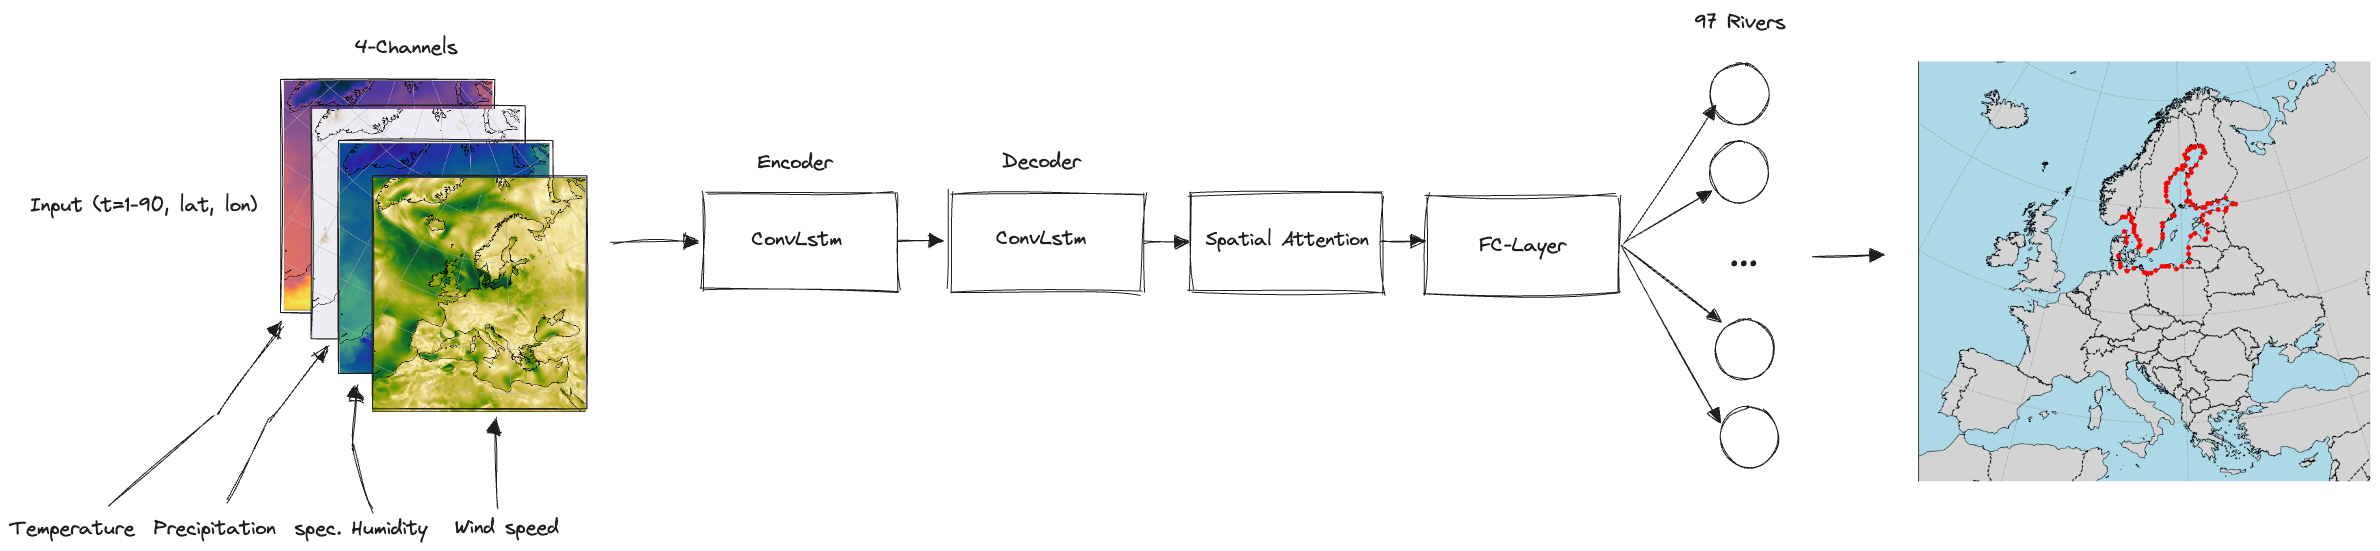
\includegraphics{model_structure.png}

}

\caption{\label{fig-baltNet}BaltConvLSTM}

\end{figure}%

For the computation we use the following set of hyper parameters:

\begin{longtable}[]{@{}ll@{}}
\caption{Hyperparameters}\label{tbl-letters}\tabularnewline
\toprule\noalign{}
Parameter name & Parameter size \\
\midrule\noalign{}
\endfirsthead
\toprule\noalign{}
Parameter name & Parameter size \\
\midrule\noalign{}
\endhead
\bottomrule\noalign{}
\endlastfoot
Channel size & 4 \\
Num. hidden layer & 10 \\
Num. timesteps & 30 \\
Conv. Kernelsize & (9,9) \\
Num. ConvLSTM layers & 1 \\
Batch size & 64 \\
~Learning Rate & 1e-3 with CosineAnnealing \\
\end{longtable}

As input the model receives 30 days of atmospheric surface fields
temperature \(T\), precipitation \(P\), specific humidity \(Q\) and wind
speed \(W\), with a daily resolution to predict the river runoff \(R\)
at the time step \(\Delta t+1\) , which can be summarized as

\(R_{\Delta t+1} = f\left(T_{t-30:t}, P_{t-30:t}, Q_{t-30:t}, W_{t-30:t}\right)\)

with f being a function maps the 30 days of daily atmospheric surface
fields data to the predicted river runoff.

The choice of atmospheric fields was based on the implemented river
runoff calculation in the atmospheric model COSMO-CLM which uses these
four fields to calculate an river runoff estimate.

\section{Results}\label{results}

For the evaluation of the model performance we consider the period 1979
to 2011. For this period no bias correction was applied to the orignal
E-HYPE dataset. We chose a split of 80\% training data, 10\% validation
data to evaluate the performance of the model during training, and 10\%
training data that is finally used to evaluate the performance of the
model after training.

The accuracy of the model is further displayed in
\textbf{?@fig-statistical-evaluationNN} . The correlation is close to 1
and the residuals show the error of the model is below 1\% of the
original data.

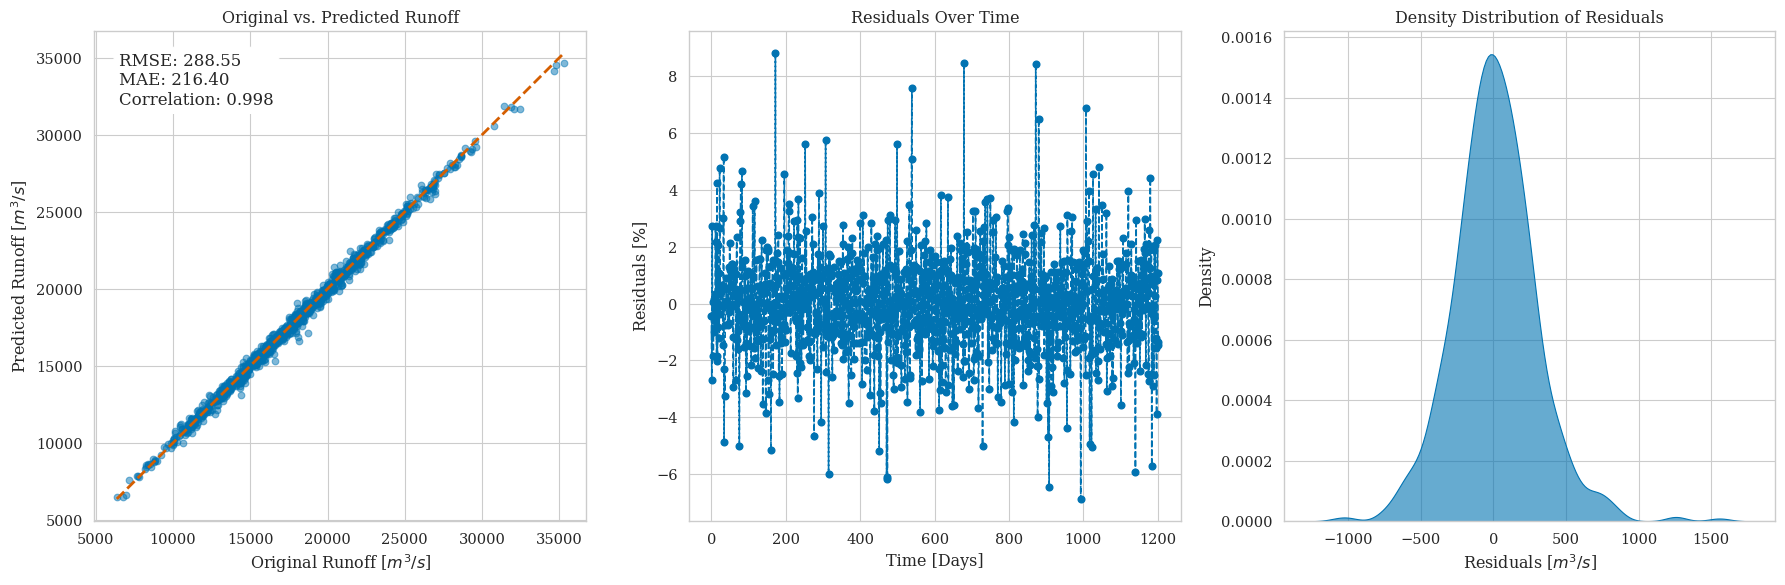
\includegraphics{images/paste-13.png}

\textbf{?@fig-PerformanceNeuralNetworkRunoff} shows the performance of
the model using the test dataset. The predicted total river runoff for
the Baltic Sea is closely matching the original data. Zooming in on the
largest individual rivers (lower panels) it can be seen that that also
the prediction of the inidivual rivers is close to the original data.

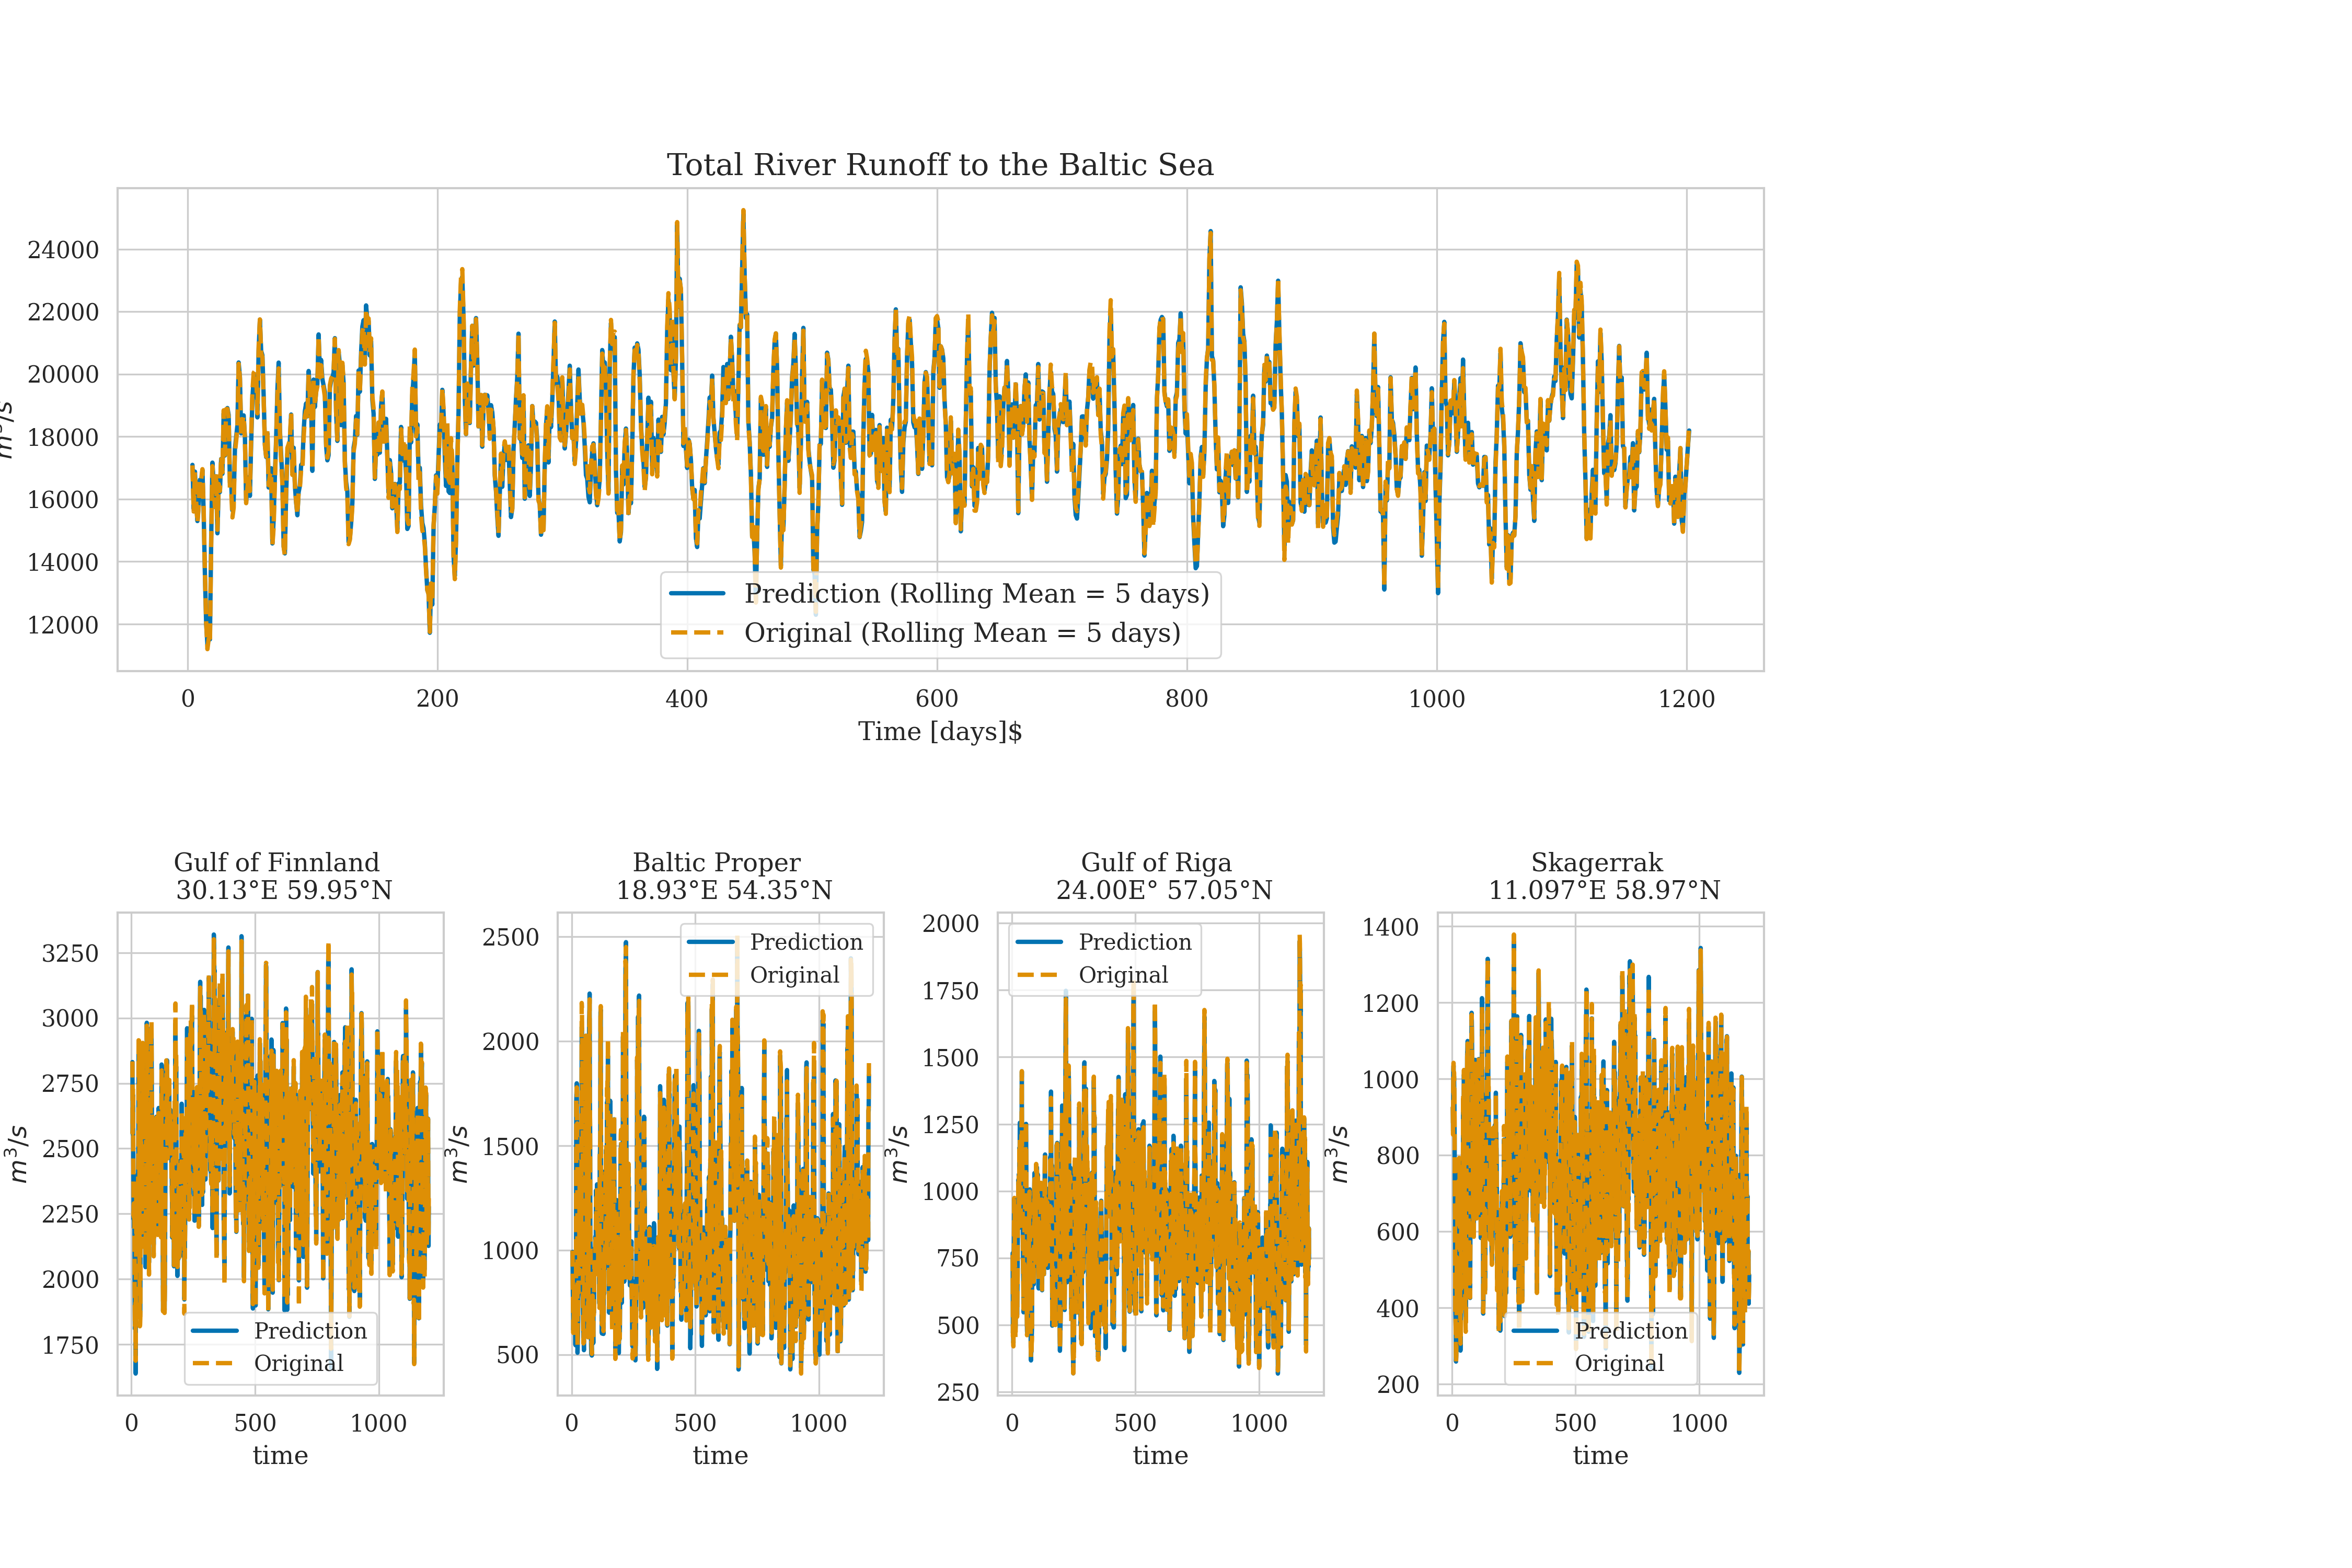
\includegraphics{images/paper_total_river_runoff.png}

Lastly, we evaluated the performance of the runoff model by
incorporating the predicted river runoff as forcing into the ocean model
MOM5. This provides a robust validation of the runoff model against more
complex real world conditions. This allows us to ensure that the
predictions accurately reflect the impact of the river discharge on the
ocean dynamics, validating the temporal and spatial variability of the
the river discharge. \textbf{?@fig-by15} shows the salinity comparison
between the original E-HYPE river runoff and the predicted river runoff
at BY15 - a central stations in the Baltic Sea.

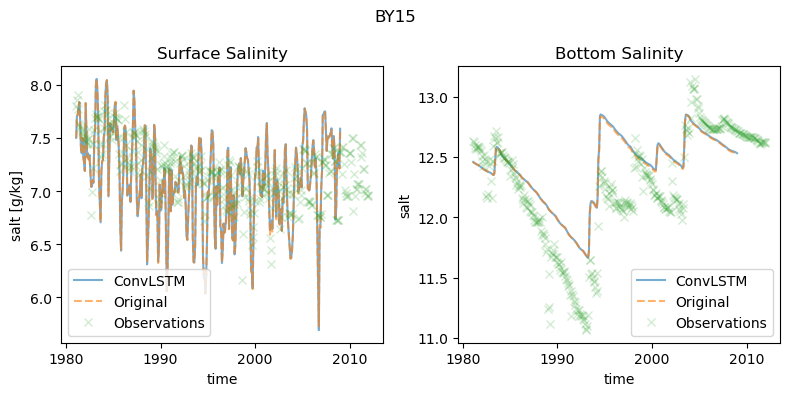
\includegraphics{images/paste-9.png}

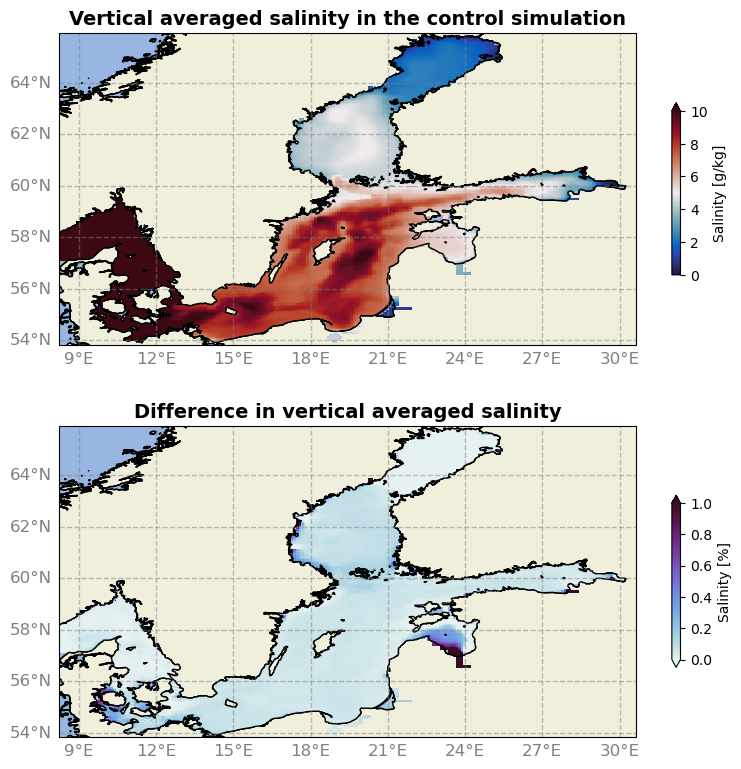
\includegraphics{images/paste-12.png}

\section{Acknowledgments}\label{acknowledgments}

Phasellus interdum tincidunt ex, a euismod massa pulvinar at. Ut
fringilla ut nisi nec volutpat. Morbi imperdiet congue tincidunt.
Vivamus eget rutrum purus. Etiam et pretium justo. Donec et egestas sem.
Donec molestie ex sit amet viverra egestas. Nullam justo nulla,
fringilla at iaculis in, posuere non mauris. Ut eget imperdiet elit.

\section{Open research}\label{open-research}

Phasellus interdum tincidunt ex, a euismod massa pulvinar at. Ut
fringilla ut nisi nec volutpat. Morbi imperdiet congue tincidunt.
Vivamus eget rutrum purus. Etiam et pretium justo. Donec et egestas sem.
Donec molestie ex sit amet viverra egestas. Nullam justo nulla,
fringilla at iaculis in, posuere non mauris. Ut eget imperdiet elit.

\section*{References}\label{references}
\addcontentsline{toc}{section}{References}

\phantomsection\label{refs}
\begin{CSLReferences}{1}{0}
\vspace{1em}

\bibitem[\citeproctext]{ref-dee2011}
Dee, D. P., Uppala, S. M., Simmons, A. J., Berrisford, P., Poli, P.,
Kobayashi, S., et al. (2011). The ERA-Interim reanalysis: configuration
and performance of the data assimilation system. \emph{Quarterly Journal
of the Royal Meteorological Society}, \emph{137}(656), 553--597.
\url{https://doi.org/10.1002/qj.828}

\bibitem[\citeproctext]{ref-fangExaminingApplicabilityDifferent2019}
Fang, W., Huang, S., Ren, K., Huang, Q., Huang, G., Cheng, G., \& Li, K.
(2019). Examining the applicability of different sampling techniques in
the development of decomposition-based streamflow forecasting models.
\emph{Journal of Hydrology}, \emph{568}, 534--550.
\url{https://doi.org/10.1016/j.jhydrol.2018.11.020}

\bibitem[\citeproctext]{ref-gruxf6ger2022}
Gröger, M., Placke, M., Meier, M., Börgel, F., Brunnabend, S.-E.,
Dutheil, C., et al. (2022). \emph{The Baltic Sea model inter-comparison
project BMIP {\textendash} a platform for model development, evaluation,
and uncertainty assessment}. Retrieved from
\url{https://gmd.copernicus.org/preprints/gmd-2022-160/}

\bibitem[\citeproctext]{ref-ha2021}
Ha, S., Liu, D., \& Mu, L. (2021). Prediction of Yangtze River
streamflow based on deep learning neural network with El
Niño{\textendash}Southern Oscillation. \emph{Scientific Reports},
\emph{11}(1), 11738. \url{https://doi.org/10.1038/s41598-021-90964-3}

\bibitem[\citeproctext]{ref-hagemannHighResolutionDischarge2020}
Hagemann, S., Stacke, T., \& Ho-Hagemann, H. T. M. (2020). High
{Resolution Discharge Simulations Over Europe} and the {Baltic Sea
Catchment}. \emph{Frontiers in Earth Science}, \emph{8}.
\url{https://doi.org/10.3389/feart.2020.00012}

\bibitem[\citeproctext]{ref-hordoir2019}
Hordoir, R., Axell, L., Höglund, A., Dieterich, C., Fransner, F.,
Gröger, M., et al. (2019). Nemo-nordic 1.0: A NEMO-based ocean model for
the baltic and north seas {\textendash} research and operational
applications. \emph{Geoscientific Model Development}, \emph{12}(1),
363--386. \url{https://doi.org/10.5194/gmd-12-363-2019}

\bibitem[\citeproctext]{ref-shi2015}
SHI, X., Chen, Z., Wang, H., Yeung, D.-Y., Wong, W., \& WOO, W. (2015).
Convolutional LSTM network: A machine learning approach for
precipitation nowcasting. In (Vol. 28). Curran Associates, Inc.
Retrieved from
\url{https://proceedings.neurips.cc/paper/2015/hash/07563a3fe3bbe7e3ba84431ad9d055af-Abstract.html}

\bibitem[\citeproctext]{ref-tanAdaptiveMiddleLongterm2018}
Tan, Q.-F., Lei, X.-H., Wang, X., Wang, H., Wen, X., Ji, Y., \& Kang,
A.-Q. (2018). An adaptive middle and long-term runoff forecast model
using {EEMD-ANN} hybrid approach. \emph{Journal of Hydrology},
\emph{567}, 767--780.
\url{https://doi.org/10.1016/j.jhydrol.2018.01.015}

\bibitem[\citeproctext]{ref-theross}
The rossby centre regional climate model RCA3: Model description and
performance - tellus a: Dynamic meteorology and oceanography. (n.d.).
Retrieved from
\url{https://a.tellusjournals.se/articles/10.1111/j.1600-0870.2010.00478.x}

\bibitem[\citeproctext]{ref-yangDerivingOperatingRules2018}
Yang, Z., Liu, P., Cheng, L., Wang, H., Ming, B., \& Gong, W. (2018).
Deriving operating rules for a large-scale hydro-photovoltaic power
system using implicit stochastic optimization. \emph{Journal of Cleaner
Production}, \emph{195}, 562--572.
\url{https://doi.org/10.1016/j.jclepro.2018.05.154}

\end{CSLReferences}



\end{document}
